\documentclass[12pt, letterpaper, twoside]{article}
\usepackage{nopageno,epsfig, amsmath, amssymb}
\usepackage{physics}
\usepackage{mathtools}
\usepackage{hyperref}
\usepackage{xcolor}
\hypersetup{
    colorlinks,
    linkcolor={blue},
    citecolor={blue},
    urlcolor={blue}
}
\usepackage{empheq}

\usepackage[letterpaper,
            margin=0.8in]{geometry}

\title{Astro 507; Problem Set 3}
\author{\textbf{Tom Wagg}}

\newcommand{\question}[1]{{\noindent \it #1}}
\newcommand{\answer}[1]{
    \par\noindent\rule{\textwidth}{0.4pt}#1\vspace{0.5cm}
}
\newcommand{\todo}[1]{{\color{red}\begin{center}TODO: #1\end{center}}}

% custom function for adding units
\makeatletter
\newcommand{\unit}[1]{%
    \,\mathrm{#1}\checknextarg}
\newcommand{\checknextarg}{\@ifnextchar\bgroup{\gobblenextarg}{}}
\newcommand{\gobblenextarg}[1]{\,\mathrm{#1}\@ifnextchar\bgroup{\gobblenextarg}{}}
\makeatother

\newcommand{\avg}[1]{\left\langle #1 \right\rangle}
\newcommand{\angstrom}{\mbox{\normalfont\AA}}
\allowdisplaybreaks

\begin{document}

\maketitle

\question{1. \textbf{Maximum photon chemical potential}}
\answer{
    For this problem I used a couple of simple things. First the blackbody equation with a nonzero chemical potential
    \begin{equation}
        B_\nu (T) = \frac{2 h \nu^3}{c^2} \frac{1}{\exp(\frac{h \nu - \mu}{k_B T}) + 1}
    \end{equation}
    where we've just inserted the $\mu$ term in the exponential. We also need to calculate $\chi^2$ for this and we do this by
    \begin{equation}
        \chi^2 = \sum_i \frac{(\text{measured}_i - \text{model}_i)^2}{\text{uncertainty}_i^2}
    \end{equation}
    So then it's just a matter of reading in the FIRAS data file, converting the (honestly baffling) units into more familiar things and calculating the $\chi^2$ over a grid of temperatures and chemical potentials. Then the maximum allowed chemical potential with a 3-$\sigma$ uncertainty is just the maximum chemical potential within $\Delta \chi^2 \approx 6.63$ of $\chi^2_{\rm min}$ (as the reading says).

    \noindent You can find the code that I used to calculate this \href{https://github.com/TomWagg/thermo_winter22/blob/tom/pset3/code/problem_1.ipynb}{in my GitHub repo} and I found that
    \begin{equation}
        \boxed{ \mu_{\rm max} \approx 3.55 \times 10^{-20} \unit{erg} \approx 1.1 \times 10^{-4} \, k_B T_{\rm CMB} }
    \end{equation}
    I also visualised this on a contour plot which you can see in the plot on the next page.
}

\question{2a. \textbf{Entropy}}
\answer{
    Let's derive the entropy for an ideal, non-relativistic Fermi gas (in terms of $V$, $z$ and $T$). For this I will follow Lecture 10. The entropy is defined as
    \begin{equation}
        S = \frac{U + PV - N \mu}{T},
    \end{equation}
    so we just need to use definitions of $U$, $P$, $N$ and $\mu$. The definitions of $\mu$ is trivial when using the fugacity
    \begin{equation}
        \mu = k_B T \ln z
    \end{equation}
    For the others, I refer to lecture 10 where we can find the definition of $n$ on slide 5
    \begin{equation}
        N = n V = \frac{2(2s + 1)}{\pi^{1/2} \lambda^3} V F_{1/2}(z)
    \end{equation}
    and the definition of $P$ on slide 7
    \begin{equation}
        P = \frac{4(2s + 1)}{3 \pi^{1/2}} k_B T \lambda^{-3} F_{3/2}(z)
    \end{equation}
    \begin{center}
        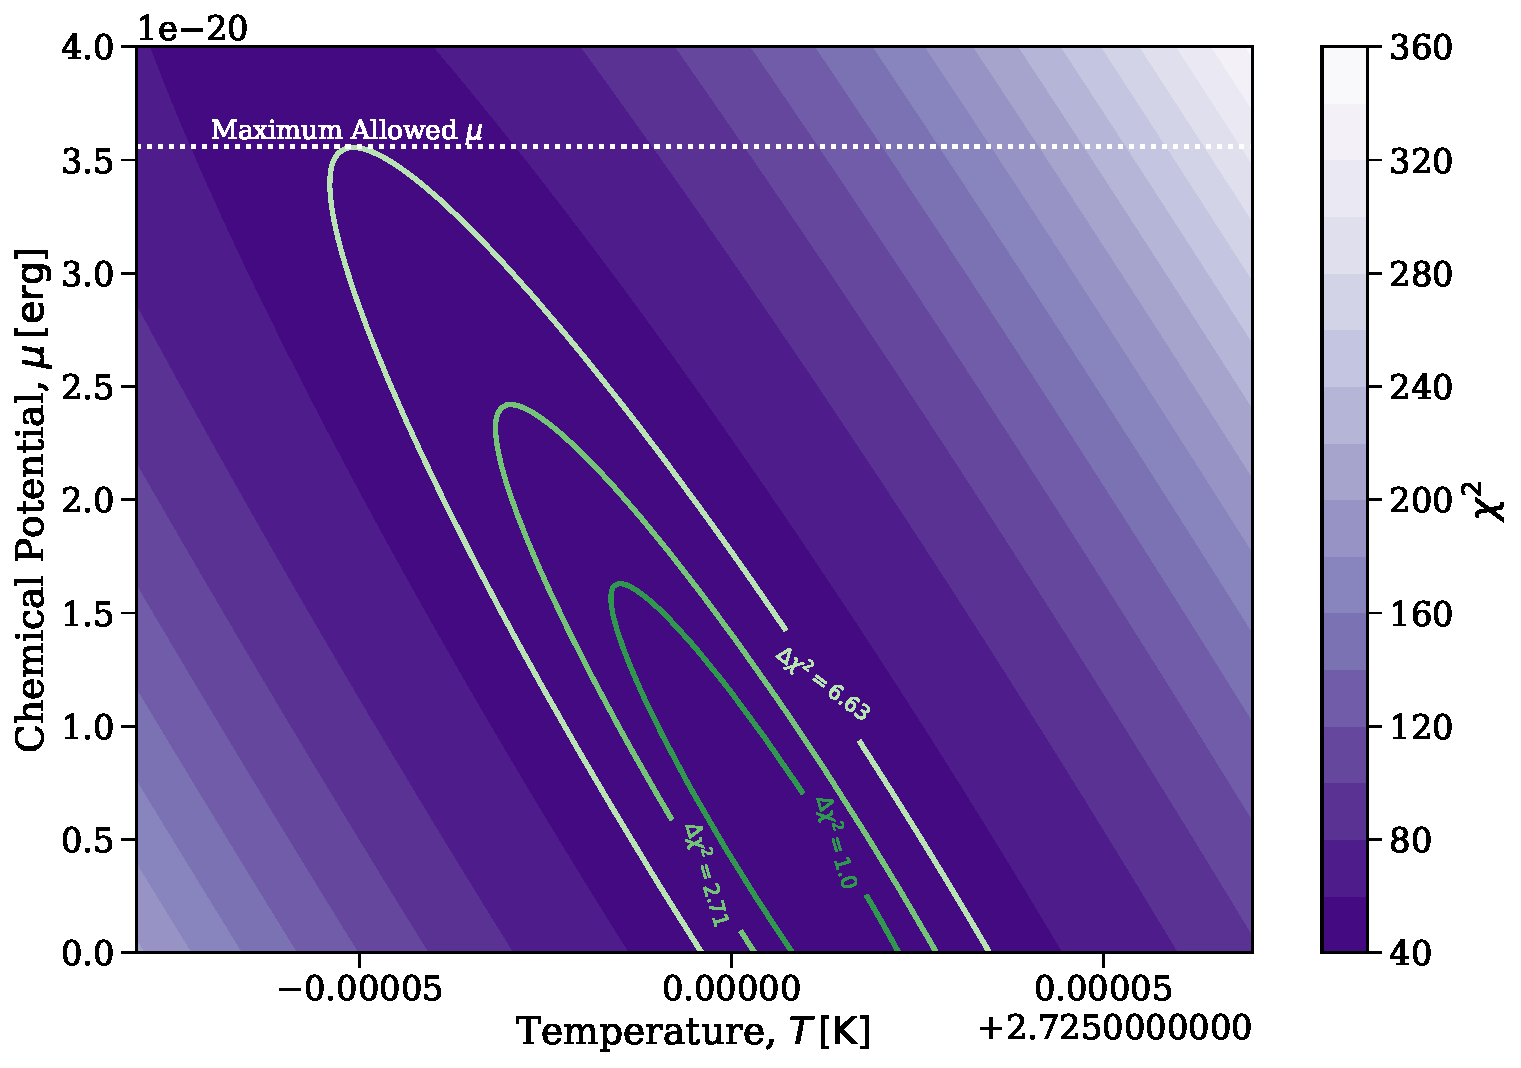
\includegraphics[width=\textwidth]{figures/max_mu.pdf}
    \end{center}
    For the total energy, we don't have it from the slides but we can derive it in the same way using Fermi-Dirac integrals. It starts in the same way as $n$ but with an extra factor of $\epsilon$ in the numerator, then we use the substitution $w = \epsilon / k_B T$
    \begin{align}
        U &= (2s + 1) \frac{V}{h^3} \int \frac{\epsilon}{e^{\frac{\epsilon - \mu}{k_B T}} + 1} \dd{\va{p}} \\
        U &= \frac{4\pi (2s + 1)}{2 h^3} (2 m k_B T)^{3/2} k_B T \int_0^\infty \dd{w} \frac{w^{3/2}}{e^w z^{-1} + 1} \\
        U &= \frac{2(2s + 1)}{\pi^{1/2} \lambda^3} V k_B T F_{3/2}(z)
    \end{align}
    Now it's simply a matter of plugging all of these into the entropy expression.
    \begin{align}
        S &= \frac{U + PV - N \mu}{T} \\
          &= \frac{1}{T} \qty[ \frac{2(2s + 1)}{\pi^{1/2} \lambda^3} V k_B T F_{3/2}(z) + \frac{4(2s + 1)}{3 \pi^{1/2}} V k_B T \lambda^{-3} F_{3/2}(z) + \frac{2(2s + 1)}{\pi^{1/2} \lambda^3} V k_B T \ln z F_{1/2}(z)] \\
          &= \frac{2(2s + 1) V k_B}{\pi^{1/2} \lambda^3} \qty[ F_{3/2}(z) + \frac{2}{3} F_{3/2}(z) + \ln z F_{1/2}(z)] \\
        \Aboxed{ S &= \frac{2(2s + 1) V k_B}{\pi^{1/2} \lambda^3} \qty[ \frac{5}{3} F_{3/2}(z) + F_{1/2}(z) \ln z] }
    \end{align}
}

\question{2b. \textbf{Expanding pressure}}
\answer{
    To start, we can right a simplified expression for $P / n k_B T$ using the expressions from part a.
    \begin{align}
        \frac{P}{n k_B T} &= \frac{4(2s + 1)}{3 \pi^{1/2}} k_B T \lambda^{-3} F_{3/2}(z) \qty[\frac{2(2s + 1)}{\pi^{1/2} \lambda^3} k_B T F_{1/2}(z)]^{-1} \\
        \frac{P}{n k_B T} &= \frac{2 F_{3/2}(z)}{3 F_{1/2}(z)}
    \end{align}
    Now we need to expand this in terms of $z$. Let's start by just expanding the Fermi-Dirac integral to start with. We know this is defined as
    \begin{equation}
        F_v(z) = \int_0^\infty \dd{w} \frac{w^v}{e^w z^{-1} + 1}
    \end{equation}
    If we perform a Taylor expansion on this we find
    \begin{equation}
        F_v(z) \approx \int_0^\infty \qty(\sum_{i = 1}^{\infty} (-1)^{i - 1} e^{- i w} w^v z^i) \dd{w}
    \end{equation}
    We can switch the order of this sum and integral and also pull out the $z$ terms to find that
    \begin{equation}
        F_v(z) \approx \sum_{i = 1}^{\infty} \qty( (-1)^{i - 1} z_i \int_0^\infty e^{- i w} w^v \dd{w} )
    \end{equation}
    Let's keep the first two terms of this (since just keeping the first results in just getting 1 as the answer haha). This gives the ratio as
    \begin{equation}
        \frac{P}{n k_B T} \approx \frac{2}{3} \frac{\frac{3 \sqrt{\pi}}{4} z - \frac{3 \sqrt{\pi}}{16 \sqrt{2}} z^2}{\frac{\sqrt{\pi}}{2} z - \frac{\sqrt{\pi}}{4 \sqrt{2}} z^2}
    \end{equation}
    Also of those factors of $\sqrt{\pi}$ cancel and we can also taylor expand again to get a nice simple expression as a function of the fugacity
    \begin{equation}
        \boxed{ \frac{P}{n k_B T} \approx 1 + \frac{z}{4 \sqrt{2}} }
    \end{equation}
}

\pagebreak

\question{\textbf{3. Brown Dwarf}}

\question{3a. \textbf{Fugacity}}
\answer{
    The general goal here is to find the number density based on the central temperature and density and then solve for the Fermi-Dirac integral and we can then invert that to find the fugacity. To start, we know that
    \begin{equation}
        \rho = m_e n_e + m_{\rm H} n_{\rm H} + m_{\rm He} n_{\rm He}
    \end{equation}
    We can rewrite this (and neglect the electron term) as
    \begin{equation}
        \rho = n_{\rm H} \qty(m_{\rm H} + m_{\rm He} \frac{n_{\rm He}}{n_{\rm H}})
    \end{equation}
    Now we can plug in the masses of hydrogen and helium as well as their relative abundance (given as 0.1 in the problem description).
    \begin{equation}
        n_{\rm H} = \frac{\rho_c}{1.4 m_p}
    \end{equation}
    Now we just relate this to the electron number density simply as
    \begin{equation}
        n = \qty(2 \frac{n_{\rm He}}{n_{\rm H}} + 1) n_{\rm H}
    \end{equation}
    And combining the two gives an expression for the number density in terms of the central density
    \begin{equation}
        n = \frac{1.2 \rho_c}{1.4 m_p}
    \end{equation}
    The other part that we need is the de-Broglie wavelength which depends on the central temperature as
    \begin{equation}
        \lambda = \frac{h}{\sqrt{2 \pi m_e k_B T_c}}
    \end{equation}
    Now let's use this with the equation for the number density from Lecture 10 and solve for the Fermi-Dirac integral (plugging in values in the final equation).
    \begin{align}
        n &= \frac{2(2s + 1)}{\pi^{1/2} \lambda^3} F_{1/2}(z) \\
        F_{1/2}(z) &= \frac{n \pi^{1/2} \lambda^3}{2(2s + 1)} \\
        F_{1/2}(z) &= \frac{\pi^{1/2}}{2(2s + 1)} \frac{1.2 \rho_c}{1.4 m_p} \qty(\frac{h}{\sqrt{2 \pi m_e k_B T_c}})^3 \\
        F_{1/2}(z) &= 2.08
    \end{align}
    I took this value and inverted it using the approximate analytic expressions from the paper (Aymerich-Humet+1981) to find the fugacity.
    \begin{equation}
        \boxed{ z = 1.65 }
    \end{equation}
}

\pagebreak

\question{3b. \textbf{Pressure}}
\answer{
    In order to calculate the pressure we need to apply the same pressure equation as 2a
    \begin{equation}
        P = \frac{4(2s + 1)}{3 \pi^{1/2}} k_B T \lambda^{-3} F_{3/2}(z)
    \end{equation}
    In this specific case, $s = 1/2$, $T = 6 \times 10^6 \unit{K}$, $\lambda$ is calculated in the same way as part a and we found that $z = 1.65$ in part a. This gives the pressure as
    \begin{equation}
        \boxed{ P = 1.92 \times 10^{16} \unit{Pa} }
    \end{equation}
}

\question{3c. \textbf{Relativistic?}}
\answer{
    In lecture we found that electrons are relativistic when their fermi momentum is such that
    \begin{equation}
        p_{\rm F} \sim m_e c
    \end{equation}
    We showed that in terms of density this was equivalent to
    \begin{equation}
        \rho_{\rm rel} \sim 2 \times 10^6 \unit{g}{cm^{-3}} \cdot \frac{\mu_e}{2 m_p}
    \end{equation}
    The last term with $\mu_e$ is going to be approximately of order unity and so, since the central density is only $325 \unit{g}{cm^{-3}}$ we have that the electrons \textbf{are} relativistic
    \begin{equation}
        \boxed{ \rho_c \ll \rho_{\rm rel} \implies \text{non-relativistic} }
    \end{equation}
}

\question{3d. \textbf{Ideal Gas}}
\answer{
    For this part we simply need to calculate the pressure assuming that it was an ideal gas. In this case
    \begin{equation}
        P_{\rm ideal} = n k_B T
    \end{equation}
    We found $n$ in part a and $T = 6 \times 10^6 \unit{K}$ and thus we can quickly plug these in to find that
    \begin{equation}
        \boxed{P_{\rm ideal} = 1.38 \times 10^{16} \unit{Pa}}
    \end{equation}
    We can therefore see that the degeneracy contributes significantly since the pressure is about 40\% larger when including degeneracy effects.
}

\pagebreak

\question{3e. \textbf{Polytropes}}
\answer{
    We are given the two following equations
    \begin{align}
        \rho_c &= 8.44 \unit{g}{cm^{-3}} \frac{M}{R^3} \\
        R M^{1/3} &= \frac{0.13}{(\mu_e F_{1/2}(z))^{2/3}}
    \end{align}
    First, let's quickly find the mass per electron in units of the proton mass, $\mu_e$, knowing that the gas is 90\% hydrogen (1 nucleon, 1 electron) and 10\% helium (4 nucleons, 2 electrons).
    \begin{equation}
        \mu_e = 0.9 \cdot 1 + 0.1 \cdot 2 = 1.1
    \end{equation}
    Now we can combine these equations to instead write that
    \begin{align}
        M &= \frac{\rho_c R^3}{8.44 \unit{g}{cm^{-3}}} \\
        R &= \qty[\frac{0.13}{(\mu_e F_{1/2}(z))^{2/3}} \qty(\frac{\rho_c}{8.44 \unit{g}{cm^{-3}}})^{-1/3}]^{1/2}
    \end{align}
    Plugging in our numbers $\mu_e = 1.1$, $z = 1.65$ and $\rho_c = 325 \unit{g}{cm^{-3}}$ to get R (and then M) gives
    \begin{empheq}[box=\fbox]{align}
        R &= 0.15 \unit{R_{\odot}} \\
        M &= 0.13 \unit{M_{\odot}}
    \end{empheq}
}

\end{document}

 